%!TEX root = ../../prace.tex

\chapter{Úvod}

V době vzniku této práce jsou velice populární hry s~otevřeným světem. Lákají hráče na obsáhlost světa a~možnost nelineárního řešení problémů a~herních úkolů. Her s~otevřeným světem najdeme nepřeberné množství v~různých herních žánrech. My se zaměříme na podmnožinu her, které kromě otevřeného světa nabízí také možnosti budování struktur a~vyžadují od hráče netriviální styl hraní, který mu umožňuje ve hře přežít. V herním průmyslu se tyto hry často označují jako \textit{sanboxové}, \textit{s budováním}, \textit{s průzkumem prostředí}, \textit{o přežití}. Autor této práce má tento typ her v~oblibě a~rád by touto prací představil svoji vizi dalšího možného rozvoje her tohoto žánru. Cílem práce by měla být implementace nového herního principu stavění, které současné herní tituly nenabízí.

\section{Charakteristika her}
V práci se budeme zabývat několika různými hrami, které však mají několik společných vlastností. Jedním ze základních konceptů je využívání herních bloků. Dalším význačným prvkem je způsob integrace herních bloků do herního prostření. Některé hry jsou celé tvořeny bloky, jiné se snaží dosáhnout vyššího stupně realismu ve hře a~bloky využívají pouze pro konstrukci různých herních objektů. Důležitým tématem této práce tedy bude rozbor systému bloků a~práce s~nimi a~popis hráčských problémů způsobených danými koncepty. V další části práce pak navrhneme a~implementujeme vlastní řešení.




\subsection{Stylizované hry}
Začněme hrami, které využívají bloků jako základního elementu celé hry. Bloky zde tvoří doslova celý svět. Mezi nejpopulárnější a~širokou veřejností nejznámější bychom měli zařadit hru \MC{}. Na obrázku z této hry \ref{fig:intro_mc} si můžeme všimnout několika zásadních faktů. Vidíme zde kostičkované listí stromů (1) či hrad na skále (2), který byl postaven z~kostiček. Taktéž slunce, měsíc a~mraky (3) jsou stylizovány do kostiček. Výrazně je kostičkovaný styl vidět na nehratelných postavách (\textit{non-playable character} -- \NPC{}) -- na obrázku ovce (4), krávy a~prasata. Stejným způsobem je pak zpracován i~hráčův charakter (5), tedy postava, kterou hráč přímo ovládá.

\begin{figure}[!ht]\centering
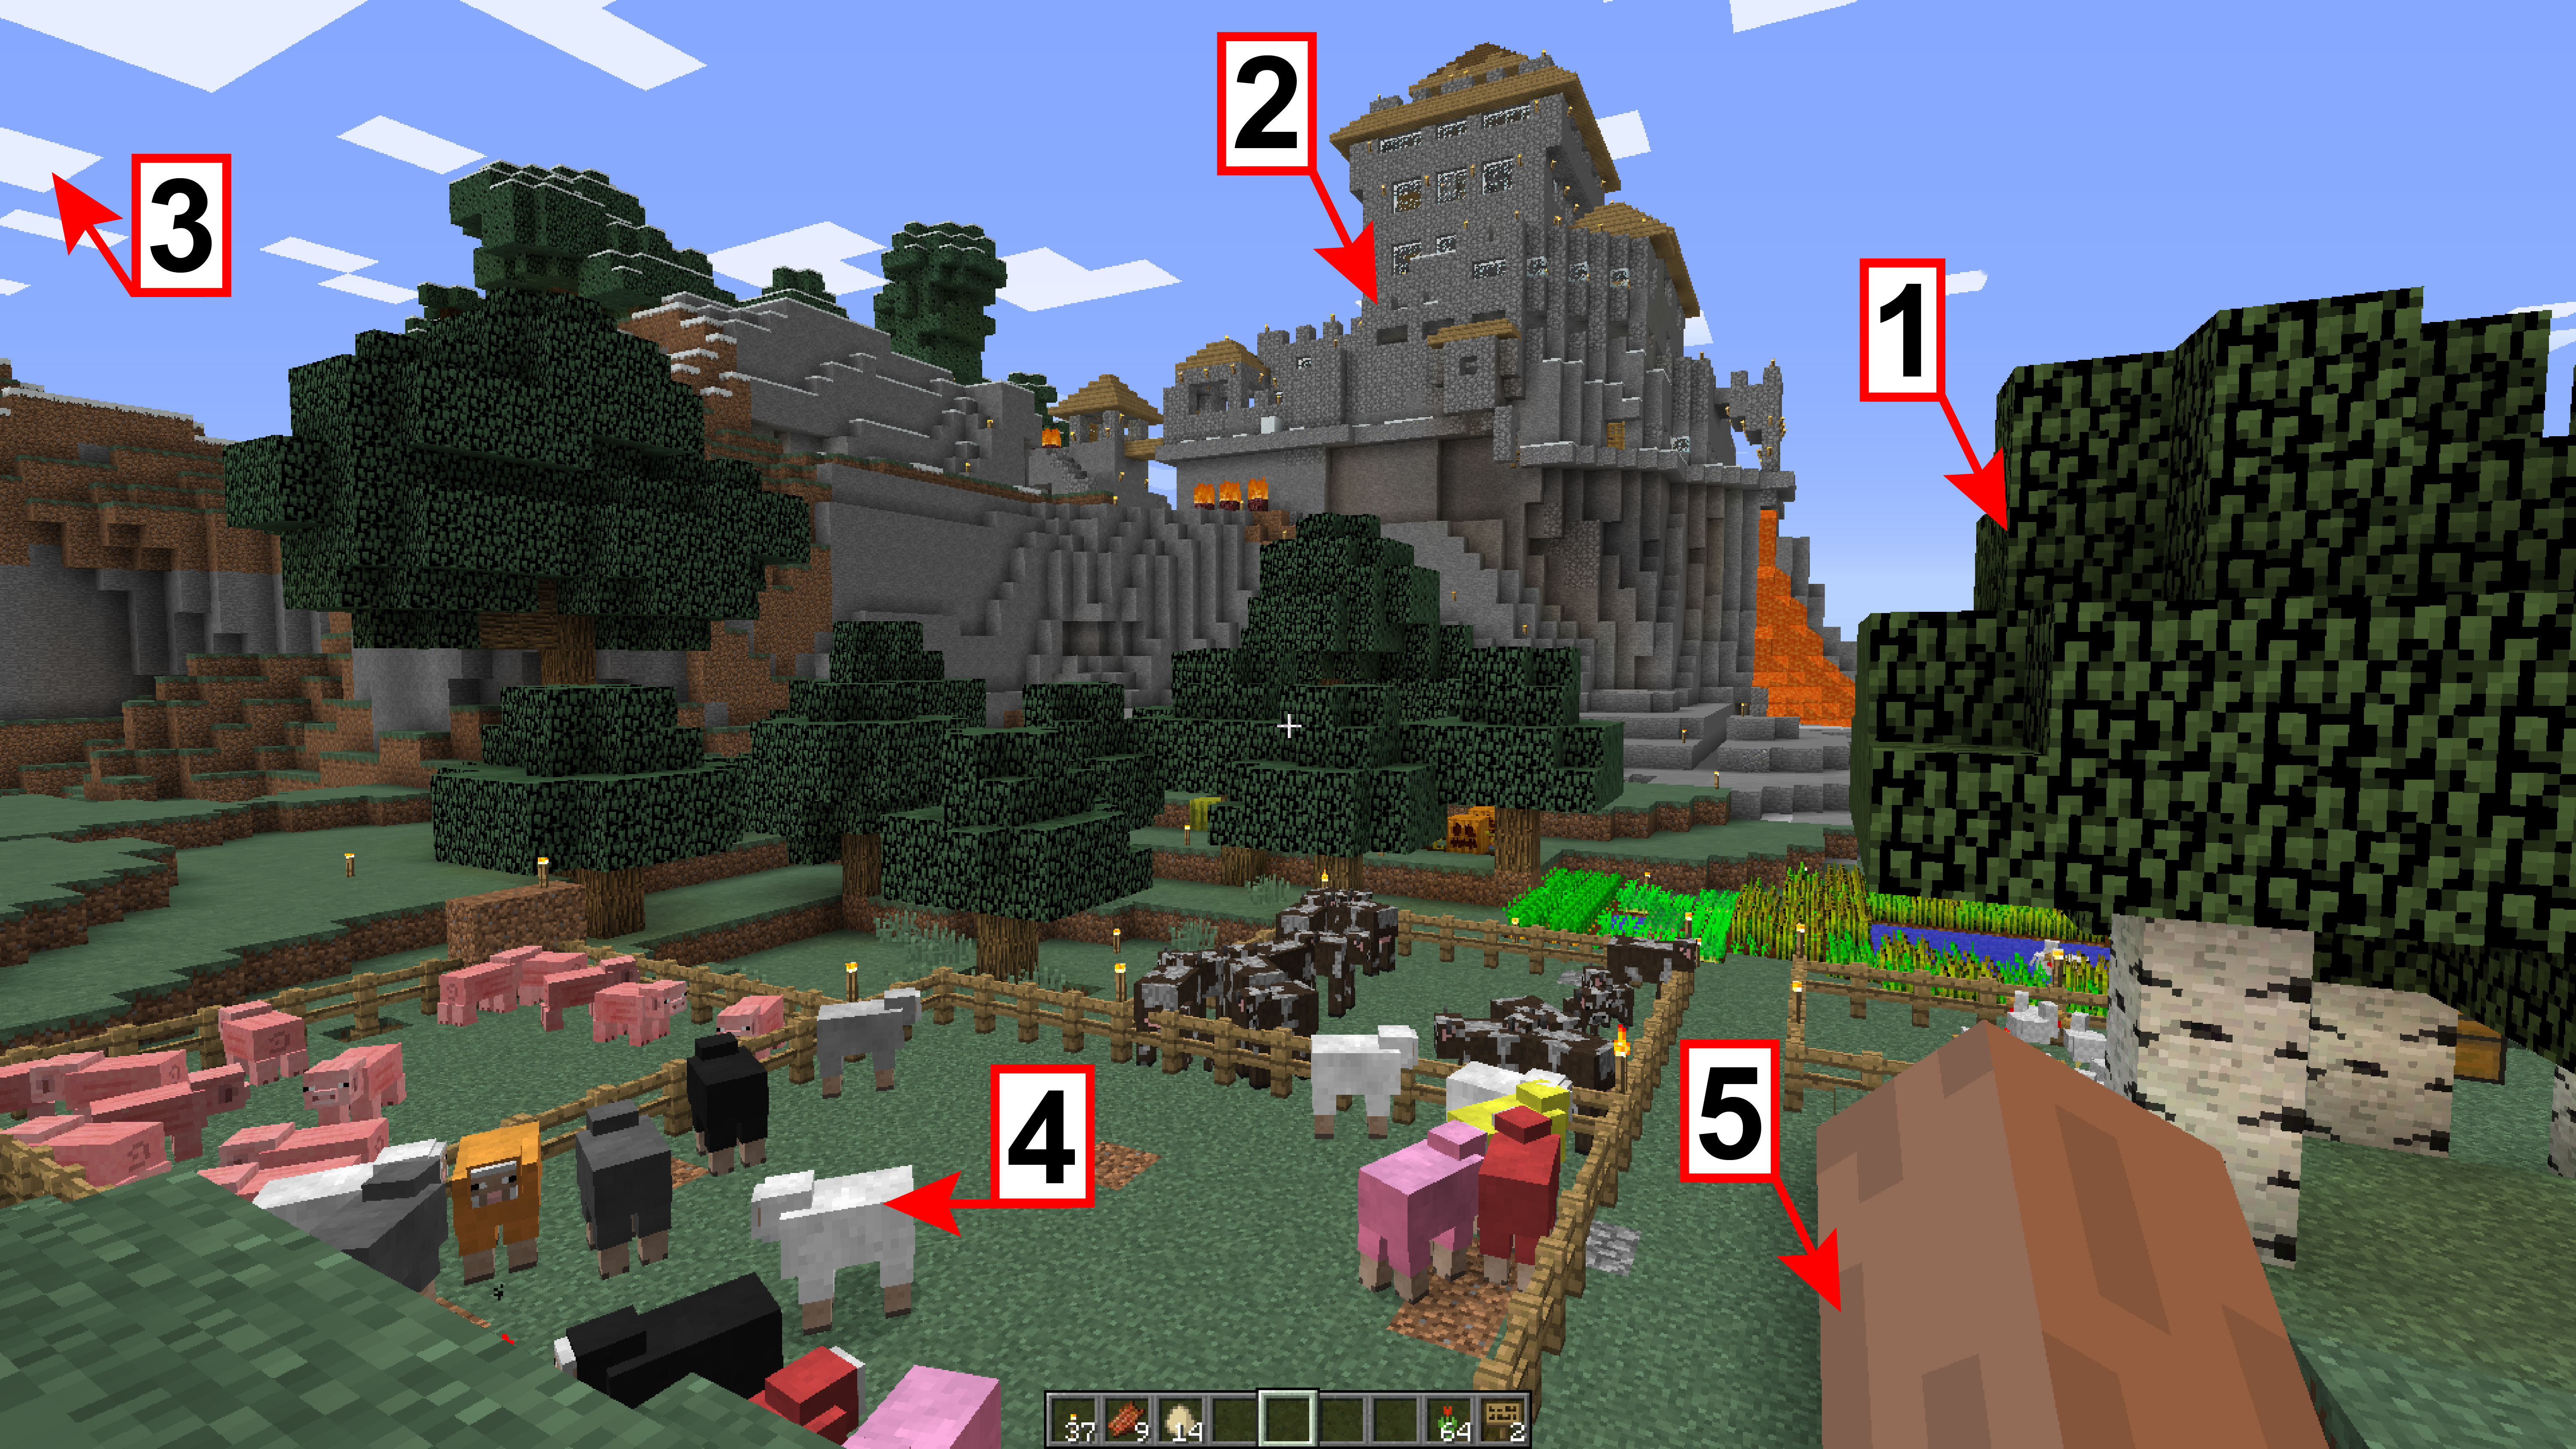
\includegraphics[ width=140mm]{../img/intro/mc}

\caption{Hra Minecraft -- hrad na skále}
\label{fig:intro_mc}

\end{figure}

\FloatBarrier

Hráč pak bloky může umisťovat do herního světa. Bloky získává těžbou (například kutáním krumpáčem do kamenného bloku), nebo je může vyrobit tzv.~\textit{Craftingem}. \textit{Crafting} probíhá skrze uživatelské rozhraní, kdy hráč z nějakých herních bloků či obecně elementů vytváří nové bloky či elementy. \MC{} používá takový systém \textit{Craftingu}, kdy hráč musí umístit bloky do konkrétního tvaru, aby získal nějaký nový objekt. Na obrázku \ref{fig:intro_crafting} můžeme vidět dvě varianty tvorby krumpáče. V jednom případě je hráčovým cílem vytvořit \textit{dřevěný krumpáč} (na obrázku vlevo), v druhém případě pak \textit{kamenný krumpáč} (vpravo). Z toho důvodu v prvním případě do vstupního tvaru umístí do horní části 3 bloky dřevěných prken, v druhém případě použije 3 bloky kamene. Tímto způsobem je možné vytvářet nejen bloky, ale i nástroje, zbraně a dokonce i jídlo, které pak hráč ve hře konzumuje.

\begin{figure}[!ht]\centering
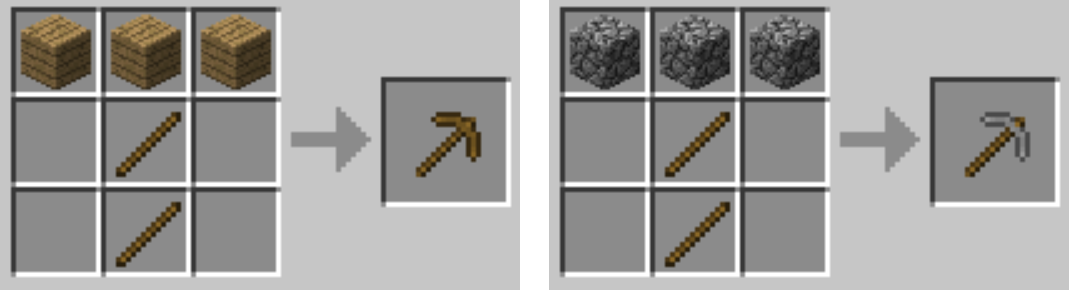
\includegraphics[ width=140mm]{../img/intro/crafting}

\caption{Hra Minecraft -- Crafting}
\label{fig:intro_crafting}

\end{figure}

\FloatBarrier

Stavění pak ve hře probíhá tak, že si hráč zvolí blok nebo objekt, který chce umístit do světa. Tento objekt musí mít ve svém inventáři. Namíří kurzor na už existující blok ve světě a klikne levým tlačítkem myši. Ke straně bloku, na který hráč mířil, se pak připojí vybraný blok. Postavený blok se odebere z inventáře a dále nevyžaduje žádnou další akci (na rozdíl od jiných her, což si ukážeme v následující sekci).


Mezi dalšími hrami bychom mohli zmínit například \TE{}. Ta je o~něco mladší než \MC{}, ale je častým zdrojem diskusí, zda je lepší new \MC{}, nebo ne. Pravdou je, že obě hry mají svůj svět kompletně složený z~kostek (\TE{} je však 2D hra), ale každá si klade trochu jiné cíle. \TE{} je více orientovaná na příběh, obsahuje více \NPC{} i~bossů. Boss je v~herní terminologii významný nepřítel, obvykle je silnější než ostatní protivníci a~velmi často bývá v~závěrečných částech hry. Duel s~bossem pak obvykle od hráče vyžaduje zjištění jeho silných a~slabých stránek a~schémat jeho útoků \citep{intro_boss}. \MC{} je pak orientován spíše na stavění. (Porovnání Minecraft vs Terraria (facts) \citep{mc_te_comparsion} na Minecraftovém fóru.)


\subsection{Hry s~prvky realismu}

Mezi hry s~prvky realismu bychom mohli zařadit třeba hry \SE{} či \ME{}, využívají kombinaci herních bloků s~\textit{voxelovou} reprezentací světa. Obě hry jsou implementovány v~proprietárním enginu společnosti Keen Software House nazvaném \textit{VRAGE}\texttrademark{}. Voxelový terén je pak v~enginu za běhu hry procedurálně generován do polygonální reprezentace, kterou pak grafická karta standardním způsobem vykreslí na obrazovce (oficiální popis vlastností enginu \citep{vrage}). Během tohoto procedurálního vytváření je na třídimenzionální strukturu voxelů (voxely si můžeme představit jako bloky stejné velikosti) aplikován nějaký šum a~tím je možné ve hře vygenerovat prakticky neomezené množství různých objektů vycházejících z~jedné voxelové struktury. \uv{\textit{The “procedural asteroids” feature adds a~practically infinite number of asteroids to the game world}} \citep{rosa_blog}. Tímto způsobem pak hry dosáhují vyššího stupně realismu -- nespoléhají se pouze na předpřipravené 3D modely, ale generují vizuální reprezentaci za běhu hry. 

Podívejme se na obrázek \ref{fig:intro_se} ze hry \SE{}. Na něm můžeme vidět převážně kamenný asteroid, a na něm je postavená vesmírná základna (obarvená zelenou barvou). K základně je přistavena větší vesmírná loď (modrobílá, v~levém horním rohu), hráč pak k~základně letí v~další, malé lodi (modrobílá uprostřed). Bližší pohled na planetku ukazuje, že její povrch není pravidelný a obsahuje spoustu nerovností (na rozdíl od tvarů základny a lodí). To je způsobeno právě algoritmickou aproximací voxelové reprezentace planetky. 

\begin{figure}[!ht]\centering
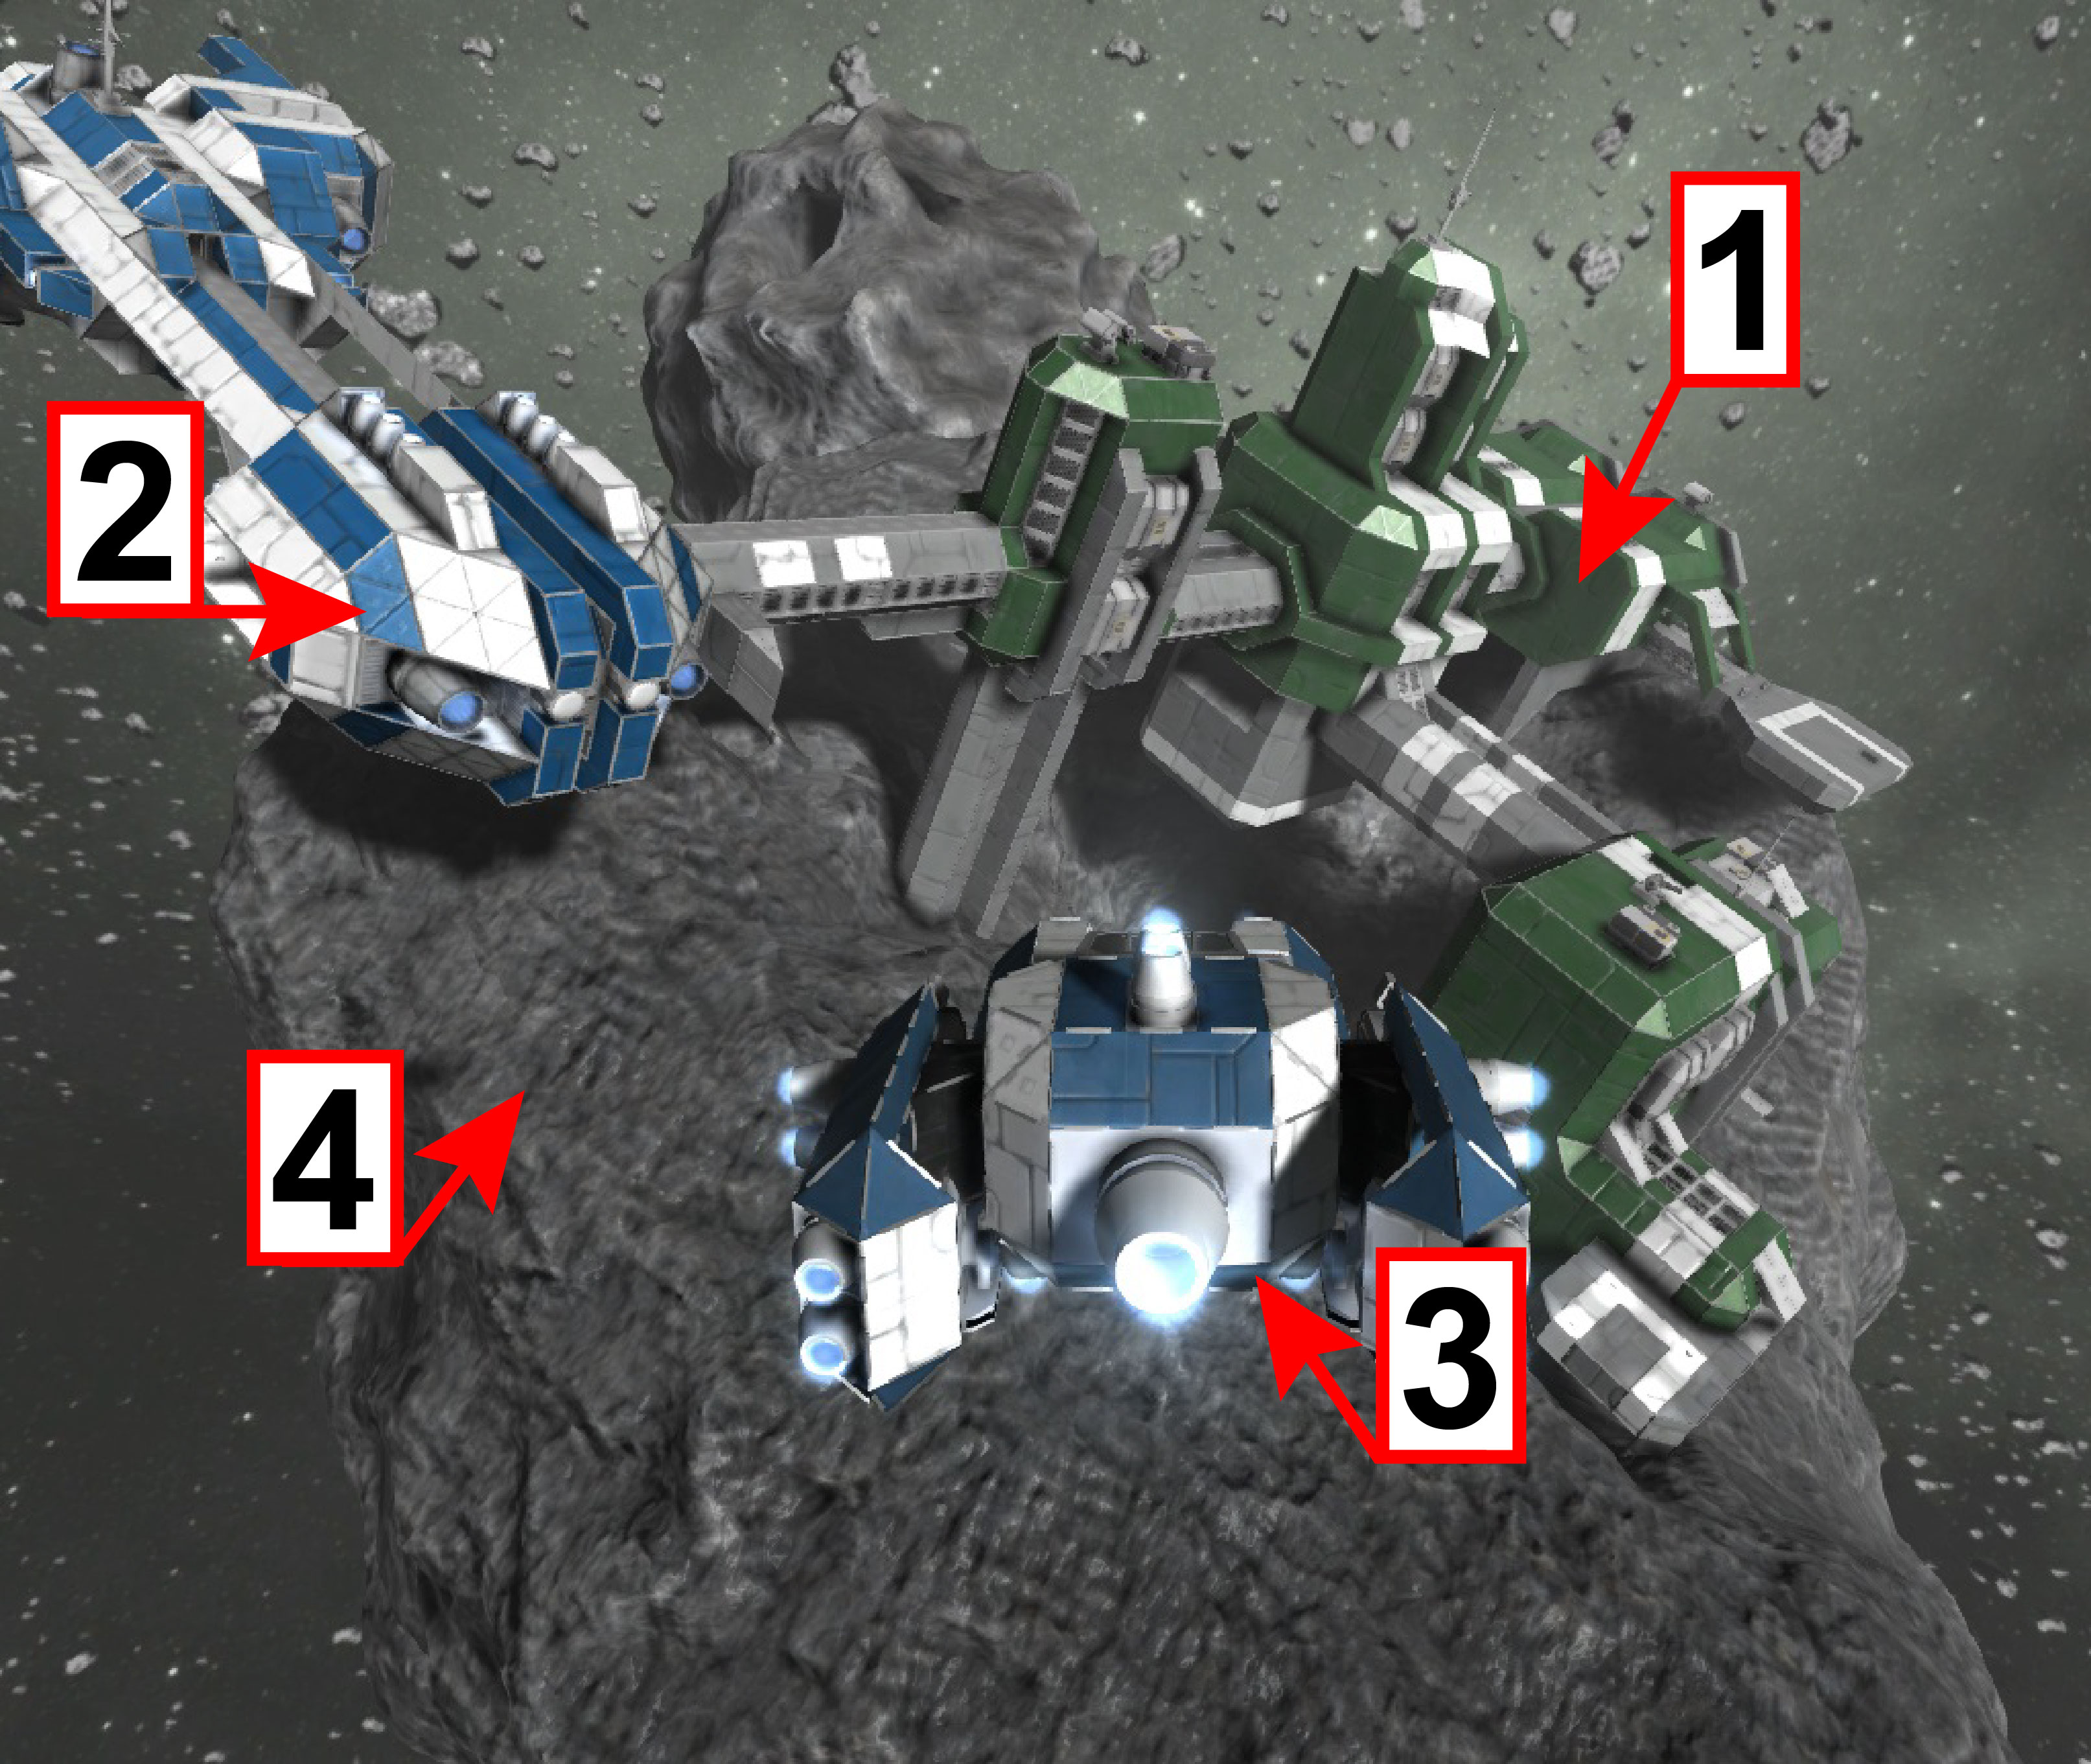
\includegraphics[ width=140mm]{../img/intro/se}

\caption{Hra Space Engineers -- základna. Zdroj: Gamespot.com \citep{se_intro_img} }
\label{fig:intro_se}

\end{figure}

\FloatBarrier

Samotná základna i~vesmírná plavidla (detailní pohled na jiné plavidlo je na obrázku \ref{fig:intro_se_ship}) jsou tvořeny bloky. Vizuální reprezentace bloku může být i~jiného tvaru než jen krychle -- to je možné vidět na obrázku \ref{fig:intro_se_blocks}). Barevně jsou zde zvýrazněny hranice bloků. Jak základny, tak vesmírné lodě (které jsou navíc oproti základnám pohyblivé) využívají tento systém. 

\begin{figure}[!ht]\centering
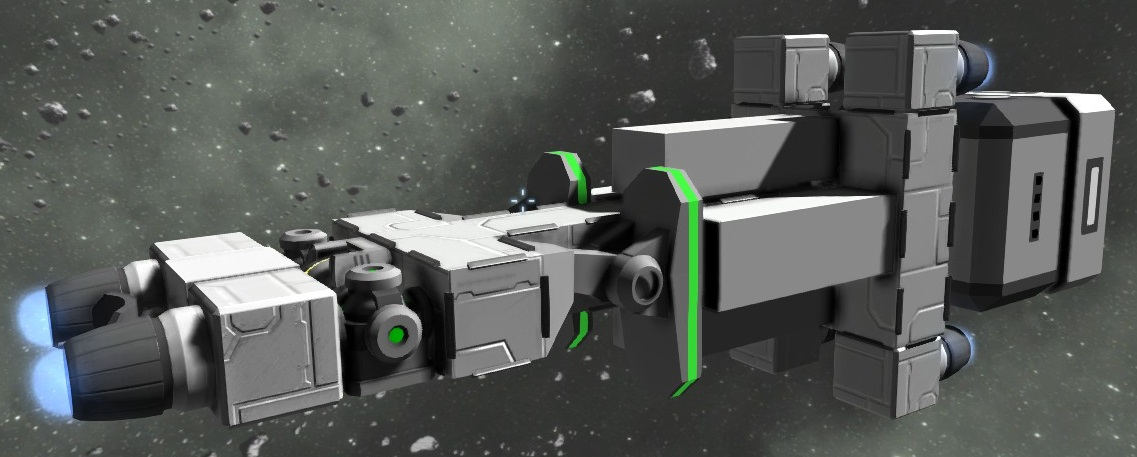
\includegraphics[ width=140mm]{../img/intro/se_ship}

\caption{Hra Space Engineers -- dron. Zdroj: space-engineer.net \citep{se_drone_source}}
\label{fig:intro_se_ship}

\end{figure}

\begin{figure}[!ht]\centering
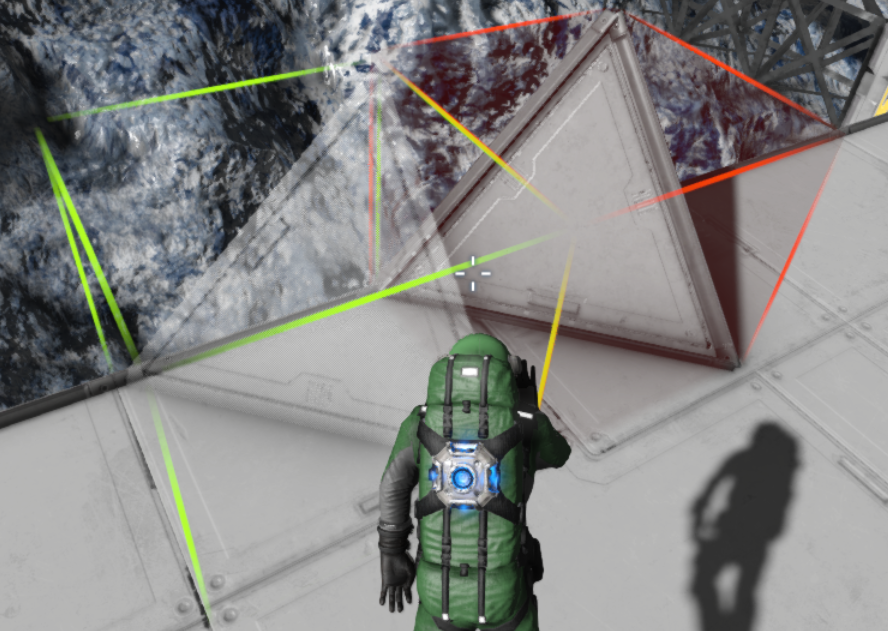
\includegraphics[ width=140mm]{../img/intro/se_blocks}

\caption{Hra Space Engineers - bloky }
\label{fig:intro_se_blocks}

\end{figure}

\FloatBarrier


\SE{} umožňuje stavět pohyblivé stroje, které si hráč postaví z~herních bloků a~ty se pak chovají jako jedna entita. Stále je na ně však aplikována fyzika, takže je možné plavidlo poškodit, nebo dokonce zničit. Tento stupeň realismu od naší hry vyžadovat nebudeme. Budeme však chtít mít ve hře bloky, jejichž model není tvaru krychle. Stejně jako v \SE{} budeme chtít, aby bylo možné bloky rotovat v libovolném směru (u bloků, u kterých to bude dávat smysl).

\textit{Crafting} v podobě, ve které je použit ve hře \MC{} se ve hře \SE{} neobjevuje, ale můžeme zde nalézt obdobný systém. Hráč musí těžit rudy, které pak dává do specializovaného stroje (bloku) na zpracování. V ovládacím rozhraní tohoto bloku si pak vybere, kterou součástku chce vytvořit. Tyto součástky jsou pak použity ke stavbě bloků (zde je zásadní rozdíl se hrou \MC{}).

Hráč si vybere z nabídky všech dostupných bloků nějaký blok, který chce postavit. V případě \SE{} se tento stavěný blok chápe spíše jako návod, jak nějaký blok postavit. Po umístění vybraného bloku do světa hráč uvidí pouze základní konstrukci vycházející z tvaru bloku. Za použití specializovaného nástroje a součástek ze svého inventáře pak po nějakou dobu \uv{staví} daný blok, přičemž v průběhu tohoto stavění se spotřebovávají součástky, které blok vyžaduje, z hráčova inventáře a zároveň se po nějakých krocích mění vizuální podoba stavěného bloku. Zároveň hráč vidí na obrazovce průběh konstrukce bloku a potřebné součástky. Můžeme tedy říct, že \textit{crafting} se ve hře \SE{} neobjevuje v podobě tvorby specifických tvarů v uživatelském rozhraní a následném získání předmětu, nýbrž v podobě získávání prostředků pro tvorbu součástek, které jsou vyžadovány pro další stavbu.

Hra \ME{} pak implementuje systém na pomezí her \MC{} a \SE{}. Hráč nemá k dispozici všechny bloky, ale musí si postavit blok Výzkumného stolu, ve kterém pak za nějakou cenu může znalost konstrukce nového bloku vyzkoumat. Z výzkumu vzejde předmět (v tomto případě svitek), který si hráč může přečíst a tím se naučí stavět nový blok. Stavba pak funguje stejně jako u \SE{}. Výhodné je, že na multiplayerovém serveru je možné tyto svitky předávat dalším hráčům a ti se pak mohou stavbu nového bloku naučit také.



\subsection{Hry s~maximálním důrazem na simulaci reality}

Do této sekce bychom mohli zařadit například vesmírný simulátor \TM{}. Tato hra si klade za cíl se maximálně přiblížit zážitku, který by mohli astronauti zažít při cestách na Měsíc a na Mars. Bloky se zde objevují v podobě standardizovaných částí budov, ale třeba vozidla jsou kompletně vymodelována a hráč je nemůže stavět ani nijak modifikovat. Představu o hře si můžeme udělat z obrázku \ref{fig:intro_tom}.

\begin{figure}[!ht]\centering
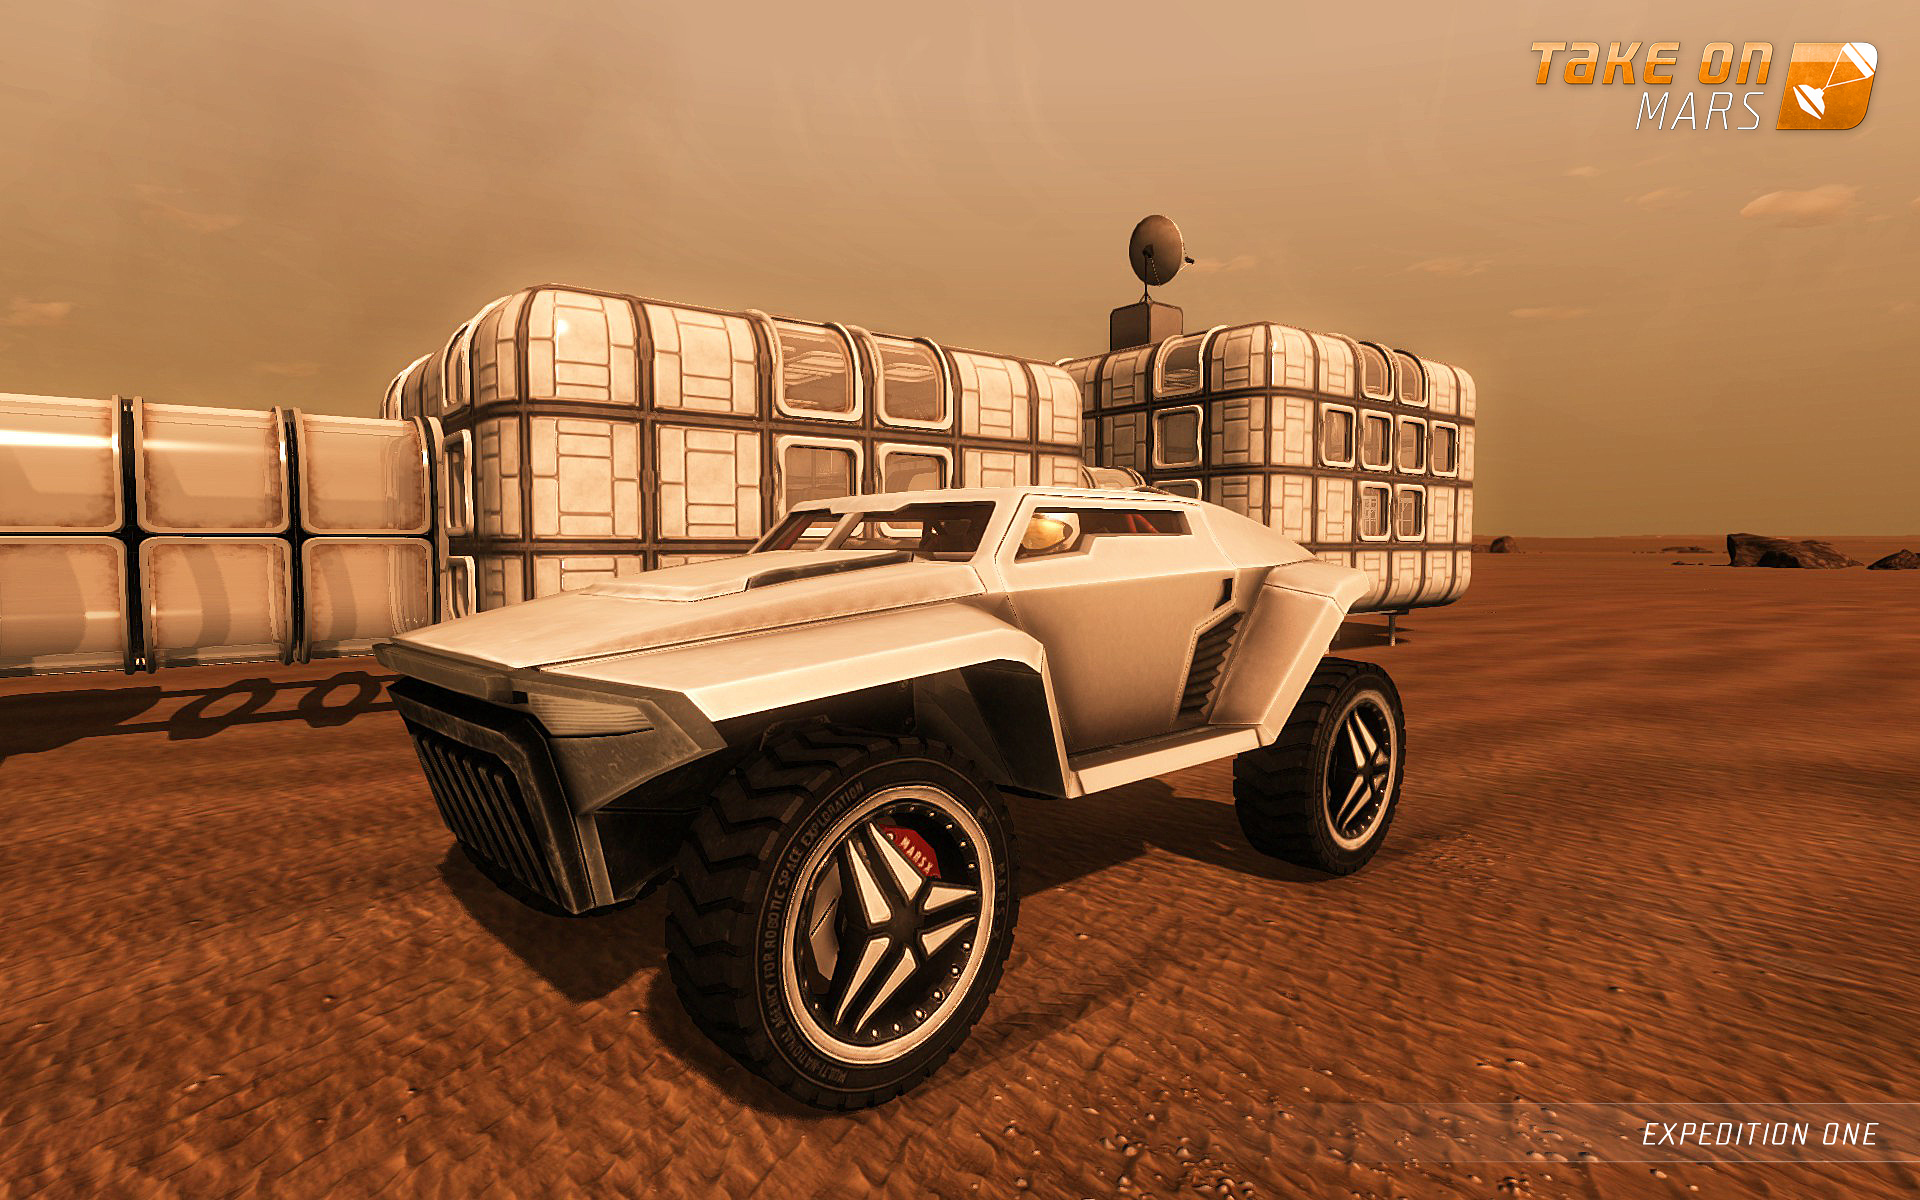
\includegraphics[ width=140mm]{../img/intro/tom}

\caption{Hry Take On Mars -- vozítko před budovou. Zdroj: Hry.cz \citep{intro_tom_source}}
\label{fig:intro_tom}

\end{figure}

\FloatBarrier

Stavění pak ve hře probíhá tak, že hráč přidává bloky k už postaveným blokům na konkrétní, vývojáři definované přípojné body. To má výhodu v tom, že hra snadno pozná, že je stavba někde \uv{děravá} a například pak neprobíhá okysličení a natlakování vnitřních prostor takovéto nedokončené stavby. Pokud bychom se rozhodli řešit vnitřní prostory stavěných budov a jejich plnění kyslíkem, tak bychom se z tohoto stylu mohli inspirovat. Hra dále nabízí možnost stavby konstruktoru objektů, kde je -- podle velikosti postaveného konstruktoru -- možné \uv{vytisknout} třeba celé vozidlo. Touto myšlenkou bychom se chtěli inspirovat. 


\subsection{Možné další inspirace }
% https://www.youtube.com/watch?v=d2ySkvn6wyw
Hra \NI{} patří do žánru \textit{MMORPG} (\textit{massively multiplayer online role-playing game} -- onlinová hra na hrdiny s velkým množstvím hráčů). Na této hře bychom rádi vypíchli koncept stavění, které probíhá poměrně netradičně. Hráč se přepne do stavitelského módu a celou stavbu si naplánuje. V tomto plánovači vidí výsledek rovnou tak, jak bude budova po dokončení vypadat. Bloky se v této fázi přichytávají do mřížky a k sobě. Po ukončení toho módu pak hráč vidí obrysy naplánovaných bloků. Pak je může začít konstruovat, přičemž v nabídce (během konstrukce) má možnost si chybějící součásti craftnout. V tomto ohledu je to tedy podobné \SE{}.


TODO dotáhnout poslední 3

%https://www.youtube.com/watch?v=Wpurqr3YaGQ 
Hra \PN{} funguje podobně jako \SE - získávání surovin, jejich crafting na komponenty a používání komponent na konstrukci objektů. Stejně tak nově postavený (ale nedokončený) objekt ukazuje základní konstrukci. Stejně jako u \SE{} je zde možné vytvářet pohyblivá vozidla, měnit terén apod. 


% https://www.youtube.com/watch?v=TOmjjo5QoP8 
\ARK{}
Ark počáteční free point, pak se bloky přidávají k sobě


\NMS{}
Stejně jako \TM{} používá snappointy

\section{Čemu se budeme věnovat}

Rádi bychom zachovali koncept použití herních bloků, který shledáváme jednoduchý na pochopení i~použití. Zaměříme se na rozšíření možnosti práce s~bloky tak, abychom uživateli nabídli, pokud možno, ještě lepší herní zážitek ze stavění vlastních výtvorů. V této práci se nebudeme nijak důkladně věnovat vizuální reprezentaci prostředí, protože ta pro nás v~tuto chvíli není podstatná. 

Změna v~přístupu k~herním blokům bude vyžadovat i~úpravy herního mechanismu s~tím souvisejícího -- hráčova inventáře. Všechny výše zmíněné hry nějakým způsobem nabízí hráči výběr bloků, které může do herního světa umístit. Naše změna by bohužel znamenala, že by se takový inventář postavitelných bloků velmi rychle stal nepřehledným a~proto musíme systém nabídky postavitelných bloků upravit pro naše potřeby.

\section{Herní bloky}



Obvykle je ve hře definován jeden základní rozměr bloku, který je neměnný. (\SE{} definuje více velikostí -- ty však nelze vzájemně kombinovat). To však může být problémem, pokud se hráč rozhodne postavit v~herním světě nějakou větší a~komplexnější strukturu podle reálné či fiktivní předlohy. Pro příklad uveďme některé výtvory ze hry \MC{} -- město Královo přístaviště z~knih Píseň ledu a~ohně od Geoge R. R. Martina, nebo hlavní město Gondoru Minas Tirith z~knih Pána prstenů od J. R. R. Tolkiena.

Autoři těchto výtvorů museli volit takové měřítko, aby byly výtvory dostatečně detailní, ale zároveň aby bylo možné výtvor postavit v~nějakém rozumném čase. Obecně můžeme říct, že čím větších detailů chtějí autoři ve hře \MC{} dosáhnout, tím větší musí celý výtvor být. To pak ale znamená, že celá stavba trvá déle, nebo je zapotřebí více spolupracujících hráčů. Hra \SE{} díky svému přístupu a~více bloků, které nejsou tvaru krychle, nabízí lepší možnosti staveb rozsáhlých objektů (představme si třeba Hvězdu smrti z~Hvězných válek), ale stále je potřeba volit nějakou rozumnou výslednou velikost. Možnosti detailů se sice zvyšují s rostoucím počtem různých vizuálních variant bloků (což je třeba případ \SE{} nebo \NI{}), ale i tak bychom chtěli navrhnout nový systém, ve kterém lze používat bloky různých velikostí.


\subsubsection{Náš návrh úpravy}
Chtěli bychom se v~této práci zabývat myšlenkou proměnlivé velikosti stavitelných bloků. Tím by hráči mohli rychleji stavět rozsáhlejší struktury a~přitom se věnovat i~drobným či estetickým detailům. Tento návrh však s~sebou nese několik problémů, které se v~této práci budeme snažit vyřešit.


\section{Inventář}
Dalším společným prvkem tohoto druhu her je inventář bloků, které může hráč umístit do herního světa. Hráč přes celé herní okno vidí \HUD{} (Head-Up Display \citep{hud_terminology}), ve kterém má zobrazenou kromě jiného nabídku bloků, které má na rychlé volbě, může je snadno zvolit a~daný blok umístit do herního světa. Navíc hry mohou definovat i~inventární skupiny bloků (\SE{}, \ME{}), mezi kterými hráč může přepínat a~tím rychle kompletně změnit sadu rychlé nabídky. Vidíme však limitaci v~tom, že hráč musí ručně spravovat tyto seznamy a~jednotlivé bloky (či nástroje) ručně umisťovat do příslušných pozic, například pomocí Drag and Drop systému (tedy přetáhnutí bloku myší z nabídky inventáře do rychlé volby stavitelných bloků.


\subsubsection{Náš návrh úpravy}
Rádi bychom navrhli jiný způsob správy těchto inventárních skupin tak, aby hráč jednou definoval, jaké prvky chce mít v~příslušných skupinách. Při vytvoření nového bloku či vytvoření jiné velikosti bloku by pak nemusel ručně přiřazovat nový blok do skupiny, ale tento blok by měl být automaticky zařazen a~nabídnut hráči.  


\section{Cíle práce}
Tato práce by měla naplnit následující cíle:
\begin{itemize}
	\item Navrhnout a~implementovat způsob řešení proměnlivé velikosti bloků
	\item Navrhnout a~implementovat automatizovanou správu inventáře
	\item Kvůli očekávaným nárokům na pochopení nových konceptů do hry implementovat základní výukový tutoriál
	\item Získat a~zhodnotit zpětnou vazbu na výslednou hru
\end{itemize}
Očekáváme však, že další cíle práce vzejdou z analýzy zadání v kapitole 2.

